\section{Definitions}
\subsection{Apache Spark}
\par  Apache Spark [3] is one of the popular open-source big
data platforms, which introduces the concept of resilient
distributed datasets (RDDs) [3] to enable fast processing of
large volume of data leveraging distributed memory. Inmemory
data operation mechanism makes it well-suited for
iterative applications such as iterative machine learning and
graph algorithms.
\par The main abstraction in Spark is resilient distributed
dataset (RDD), which represents a read-only collection of
objects distributed across a set of machines. Users can
explicitly cache an RDD in memory across machines and
reuse it in multiple MapReduce-like parallel operations. RDDs
achieve fault tolerance through a notion of lineage: if a
partition of an RDD is lost, the RDD has enough information
about how it was derived from other RDDs to be able to
rebuild just that partition. Although RDDs are not a general
shared memory abstraction, they represent a sweet-spot
between expressivity on the one hand and scalability and
reliability on the other hand, and we have found them wellsuited
for a variety of applications. The framework of Spark
cluster is shown in Figure 1.
\par
\begin{figure}[h]
	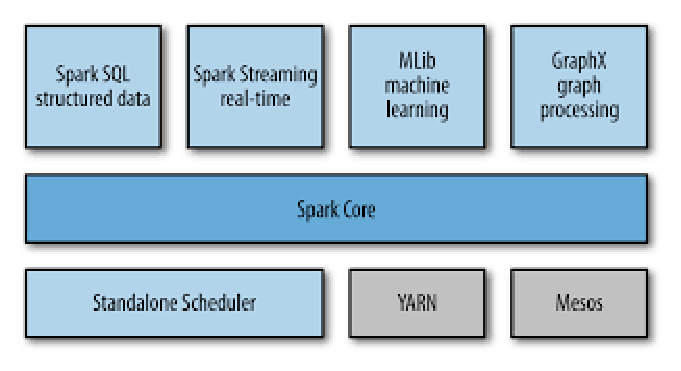
\includegraphics[width=8cm]{1.eps}
	\caption{Architecture of Apache Spark.}\label{fig:ArchitectureSpark}
\end{figure}

\begin{figure}
	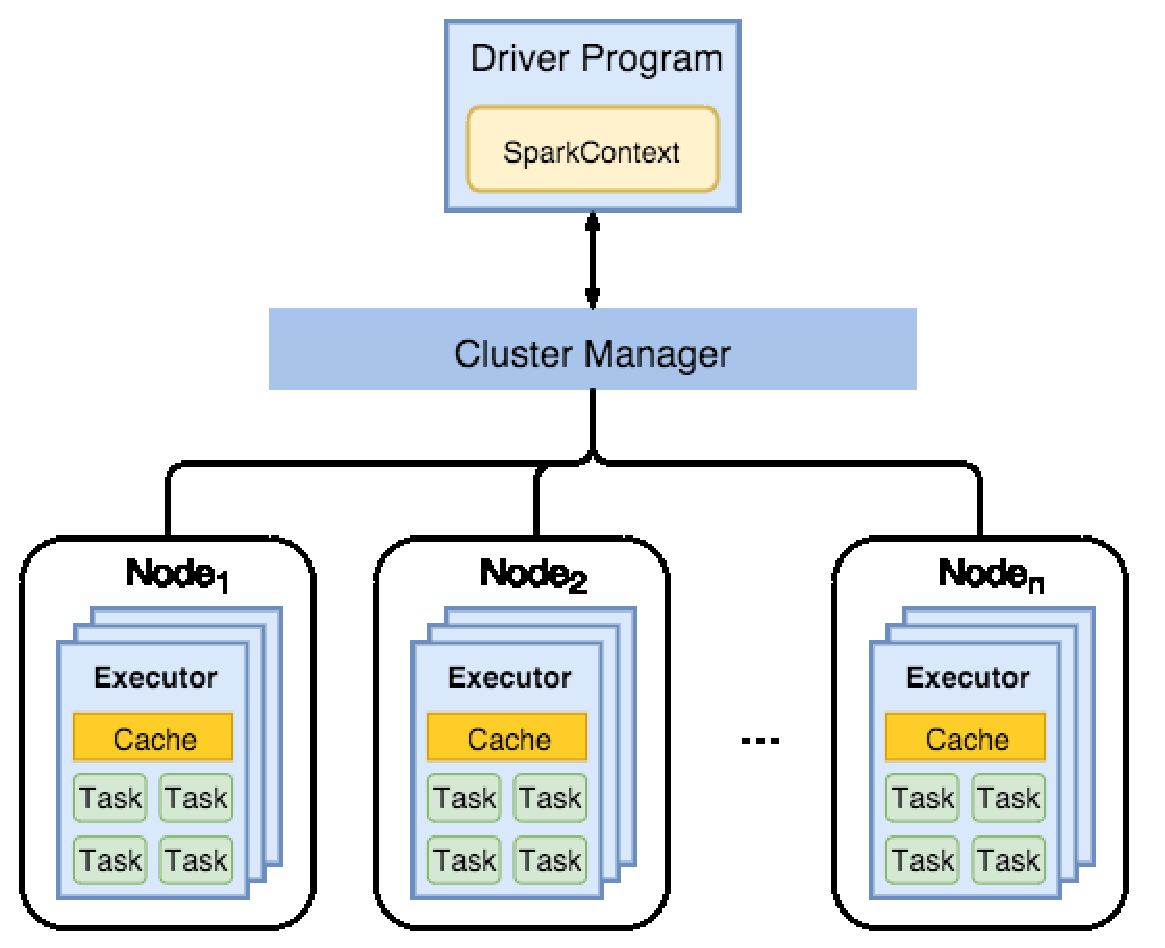
\includegraphics[width=8cm]{2.eps}
	\caption{Workflow of Spark}\label{fig:WorkflowSpark}
\end{figure}

\begin{figure}
	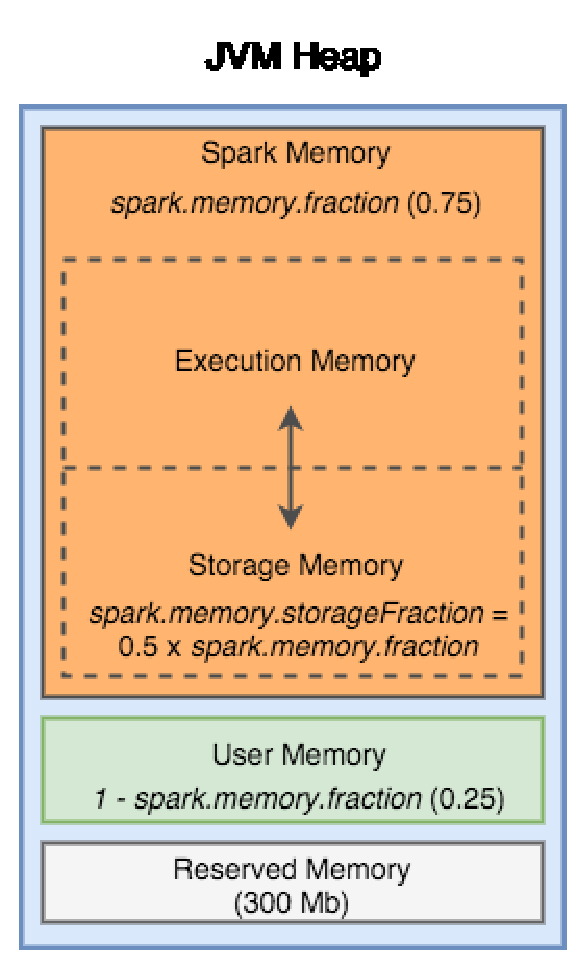
\includegraphics[width=8cm]{3.eps}
	\caption{Parameters of JVM Heap}\label{fig:ParametersJVM}
\end{figure}

\begin{figure}
	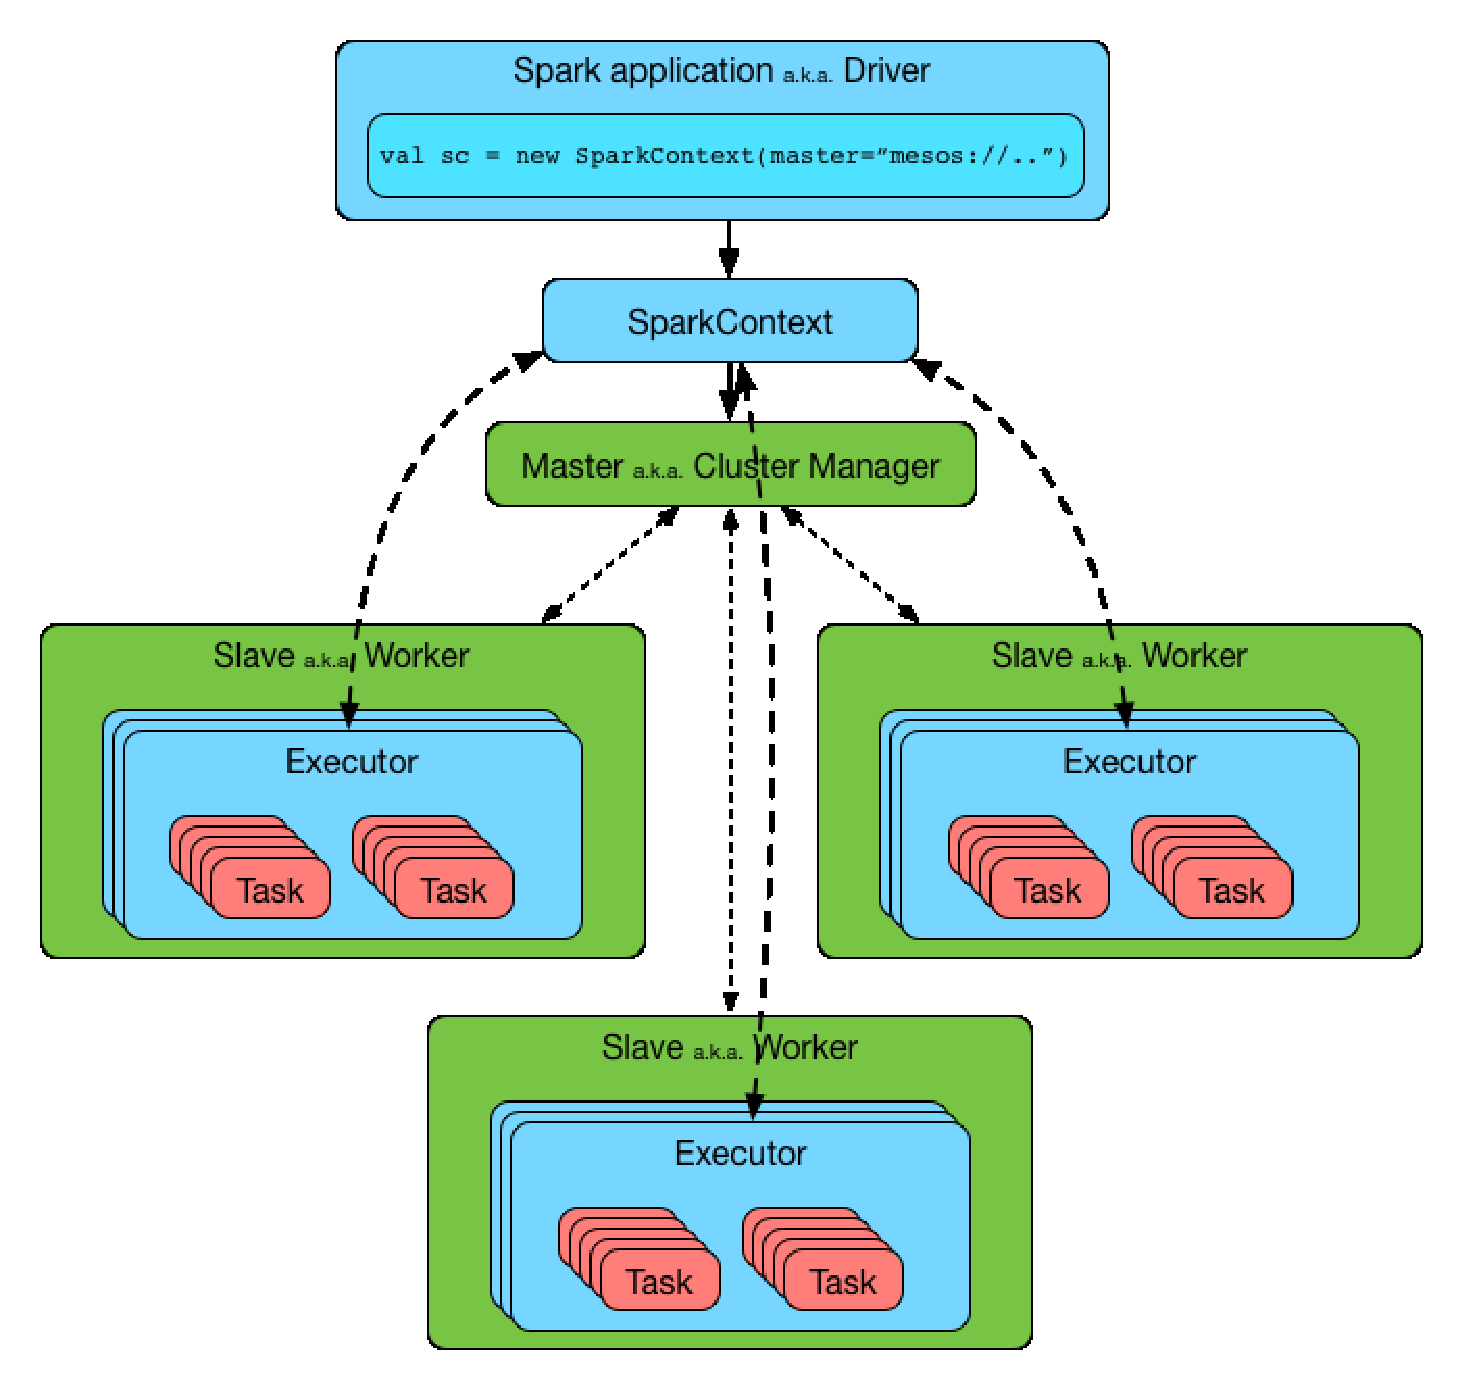
\includegraphics[width=8cm]{4.eps}
	\caption{Running of Spark}\label{fig:RunningSpark}
\end{figure}


\subsection{Definitions}

